\section{Comparisons}
\label{Comparisons}


After testing the models with different amounts of data and starting probability, we came up to some conclusions in terms of the speed and efficiency of these models. In order to be fair between agents, we tried the models with the beginning probability of 50\% (After that, we tried with 75\% as well). That way, approximately half of the data will consist of "A", and the other half will be "B". And since the selection process will take millions of times, we did not want to have a file for each iteration. Therefore, we created an output file showing the current situation using some discrete spaces. For example, we created one file for a million iterations. And of course while analyzing the data, we considered those frequencies. Here are some of our findings:\\

\underline{1 Million Agents}

Based on iteration times, 2-Choices and 3-Majority models showed a similar performance, where the consensus was obtained in around 14,000,000 iterations. While the Undecided State Dynamics model took over 21,000,000 iterations to reach a consensus. The difference may stem from that in the Undecided Model, it takes more steps for an agent to change her idea. However, as we will see for the other numbers of agents, iteration time is not enough to determine the efficiency of a model. On the contrary, it may be misleading.
We can see that in the plots based on time. When it comes to time efficiency, the Undecided Model is much more efficient than the others, with 27,000 ms. While the 2-Choices Model took almost 900,000 ms, and the 3-Majority took 600,000 ms to reach the consensus. In this sense, it is seen that for 1 Million Agents and 0.5 starting probability, the Undecided Model is over 20 times more efficient than the other models.\\


\underline{10 Million Agents}
When we increased the number of agents to 10 million, the Undecided Model still got the highest number of iterations with 350,000,000. Whereas other two models got a similar iteration time, which is around 300,000,000. In this test, the ratio between the Undecided Model and the other models was not as significant as the 1 Million Agents trial. But the Undecided Model still kept its place.
Similarly, when it comes to time comparison, the Undecided Model was still the fastest one with 2,500,000 ms. While the other two models took around 4,000,000 ms to reach the consensus.\\


\underline{100 Million Agents}
When we increased the number of agents to 100 million, the pattern did not change and the Undecided Model got the maximum value for the number of iterations; and the minimum value for the time. The time taken was 14 million ms for 3-Majority, 17.5 million ms for 2 Choice, and less than 2.5 million ms for the Undecided Model.

\begin{figure}[H]
    \centering
    \includegraphics[width=0.69\textwidth,height=0.12\textheight]{img/svg/ComparisonTime.png}
    \caption{Times (ms) of the simulations with probability to choose A equal to 0.5}
\end{figure}

\begin{figure}[H]
    \centering
    \includegraphics[width=0.67\textwidth,height=0.12\textheight]{img/svg/0.75/ComparisonTime.png}
    \caption{Times (ms) of the simulations with probability to choose A equal to 0.5}
\end{figure}